\documentclass[11pt]{article}
%DECLARATIONS
\usepackage{graphicx}
\usepackage{xcolor}
\usepackage{placeins}
\usepackage{enumitem}
\usepackage{minted}
\usepackage{hyperref}
%\usepackage[dvipsnames]{xcolor}
\usepackage{fancyvrb}
\usepackage{tcolorbox}
\usepackage{tikz}
\usetikzlibrary{shapes.multipart, calc}
\renewcommand\familydefault{\sfdefault}
\usepackage{tikz-dependency}
\usepackage{moreverb}
\usepackage[linguistics]{forest}
\usepackage{changepage}
\usepackage{float}
\usepackage{caption}
\usepackage{subcaption}
\usepackage{tikz}
\usetikzlibrary{shapes,positioning,calc}
\colorlet{lightgray}{gray!20}

\usepackage{xcolor,listings}
\usepackage[normalem]{ulem}

\definecolor{codegreen}{rgb}{0,0.6,0}
    \definecolor{codegray}{rgb}{0.5,0.5,0.5}
    \definecolor{codepurple}{HTML}{C42043}
    \definecolor{backcolour}{HTML}{F2F2F2}
    \definecolor{bookColor}{cmyk}{0,0,0,0.90}  
    \color{bookColor}

    \lstset{upquote=true}

    \lstdefinestyle{mystyle}{
        backgroundcolor=\color{backcolour},   
        commentstyle=\color{codegreen},
        keywordstyle=\color{codepurple},
        numberstyle=\footnotesize\color{codegray},
        stringstyle=\color{codepurple},
        basicstyle=\footnotesize,
        breakatwhitespace=false,         
        breaklines=true,                 
        captionpos=b,                    
        keepspaces=true,                 
        numbers=left,                    
        numbersep=-10pt,                  
        showspaces=false,                
        showstringspaces=false,
        showtabs=false,      
    }
    \lstset{style=mystyle} 
    
\newlist{MyIndentedList}{itemize}{4}
\setlist[MyIndentedList,1]{%
    label={},
    noitemsep,
    leftmargin=0pt,
    }
\setlist[MyIndentedList]{%
    label={},
    noitemsep,
    }
    
\depstyle{lvl}{%
    edge height=2.5ex,
    % edge unit distance=#1*2.5ex, % Another way of controlling the appearance of the edges.
    edge below,
    edge horizontal padding=0,
    edge vertical padding=(#1-1)*3ex,
    text only label, % No need for label for functional dependencies.
    edge slant=0, % Right angles
    rounded corners=0,
    edge style={>=triangle 60} % Change the style of the arrowheads.
}
\tikzset{
    matrix/.append style={column sep=0.4cm} % Adding some distance between the attributes.
}
\tikzstyle{TxtBook}=[% Style to mimic the textbook Fundamentals of Database Systems.
    column sep=0cm, % No distance between two attributes.
    nodes={%
        fill=gray!20,
        draw=black,
        inner xsep=3ex,
        inner ysep=1ex
    }
]

\parskip1.5ex
\addtolength{\baselineskip}{+.1\baselineskip}
\newlength{\lineheight}
\setlength{\lineheight}{11pt}
\newcommand{\ls}[1]{\baselineskip=#1\lineheight}
\newcommand{\bitem}{\begin{itemize}}
\newcommand{\eitem}{\end{itemize}}
\newcommand{\benum}{\begin{enumerate}}
\newcommand{\eenum}{\end{enumerate}}
\newcommand{\bdesc}{\begin{description}}
\newcommand{\edesc}{\end{description}}
\newcommand{\comment}[1]{{\color{red}{#1}}}

\usepackage{xcolor}
\usepackage[colorlinks = true,
            linkcolor = blue,
            urlcolor  = blue,
            citecolor = blue,
            anchorcolor = blue]{hyperref}

\newcommand{\MYhref}[3][blue]{\href{#2}{\color{#1}{#3}}}%

% redefine \VerbatimInput
\RecustomVerbatimCommand{\VerbatimInput}{VerbatimInput}%
{fontsize=\scriptsize,
 %
 commandchars=\|\(\), % escape character and argument delimiters for
                      % commands within the verbatim
 commentchar=*        % comment character
}

\newmintedfile[inputsql]{sql}{%
    linenos,
    autogobble,
    breaklines,
}

\newlist{MyIndentedList}{itemize}{4}
\setlist[MyIndentedList,1]{%
    label={},
    noitemsep,
    leftmargin=0pt,
    }
\setlist[MyIndentedList]{%
    label={},
    noitemsep,
    }
    
%BEGIN
\begin{document}
\title{Database Final Project}
\date{\today}
\author{Sahba Tashakkori and Jered Dominguez-Trujillo}

\maketitle
\pagenumbering{gobble}
\begin{center}
\end{center}
\newpage
%\pagestyle{empty}
\tableofcontents
\pagenumbering{arabic}

\pagebreak

\section{Changes Since Proposal}
\noindent
Due to the fact that the 3 data sources, fatality by age, fatality by sex, and fatality by co-morbidity, were gathered only from New York State, not updated frequently, and not comprehensive, we decided to exclude them. Additionally, we decided to exclude the US Tests dataset provided by the API since it was redundant and only provided the total number of tests done nationally, which was found to be redundant and not useful for a state-level analysis. Instead, we focused on the remaining 4 data sources from the  \MYhref{https://www.npmjs.com/package/covid19-api}{Covid-19 API}. They are listed below:

\begin{itemize}
    \item \MYhref{https://www.npmjs.com/package/covid19-api}{Covid-19 API}
        \begin{itemize}
        \item \textbf{John Hopkins Data Daily Report}: Data for the 2019 Novel Coronavirus Visual sourced from the Dashboard operated by the Johns Hopkins University Center for Systems Science and Engineering. Updated daily.
        %\item \textbf{Tests in US}: Data from 48 states public health labs in the United States, in addition to New York City, USAF, and 9 California counties. Updated daily.
        \item \textbf{USA Medical Aid Distribution}: Tracks medical aid to US hospitals and facilities, including package weight, cost, delivery date of aid to a location and/or hospital. Updated daily.
        \item \textbf{Aggregated Facility Capacity County}: Current population, (occupied) hospital beds, (occupied) ICU beds, healthcare staff, age demographics, grouped by county for the United States. Updated daily 
        \item \textbf{United States Cases By State}: For every state: the number of positive and negative cases, each state's score, number of patients in the ICU and on ventilators, and number of patients who have recovered (supplements the JHU Daily Report with additional fields).
    \end{itemize} 
\end{itemize}

\pagebreak

\section{Introduction}
\label{sec:Intro}
\noindent
Data on global and United States coronavirus (COVID-19) statistics, medical aid, facilities, and demographics will be gathered and organized into a relational database for the eventual purpose of analysis in order to understand the trends and relationships between demographics, testing, geography, hospital systems/availability, medical aid, and political response to the spread and deadliness of the coronavirus. To do this, several sites and APIs that gather and provided updated timeseries data about the coronavirus were studied and evaluated, including \MYhref{https://www.worldometers.info/coronavirus/}{Worldometer}, \MYhref{https://coronavirus.jhu.edu/map.html}{John Hopkins Coronavirus Resource Center}, \MYhref{https://covidtracking.com/api}{The Covid Tracking Project}, and an open source \MYhref{https://www.npmjs.com/package/covid19-api}{Covid-19 API}. 

\noindent
The open source \MYhref{https://www.npmjs.com/package/covid19-api}{Covid-19 API} was chosen, and several data items from the API were utilized to design a database to store time series data relating to COVID-19. The database was then used for some basic analysis and demonstration of queries. The approach taken in choosing which data to source and how it was sourced is presented in Section \ref{sec:approachsec}. The process of database design, from conceptual schema, to ER diagram, and finally the translation of the ER diagram to the relational model and implementation in Oracle Cloud DBMS is described in Section \ref{sec:designimplementation}. Finally, we present and describe some analyses and regression models that we developed using the data extracted from the designed database in Section \ref{sec:analysis}.

\section{Data Selection}
\label{sec:approachsec}

\noindent
The data sources outlined in \textbf{Section \ref{sec:Intro}} each had unique data: \MYhref{https://www.worldometers.info/coronavirus/}{Worldometer} provides updated positive cases and deaths on a rolling 24-hour basis grouped by country, \MYhref{https://coronavirus.jhu.edu/map.html}{John Hopkins Coronavirus Resource Center} provides geographical data updated frequently, \MYhref{https://covidtracking.com/api}{The Covid Tracking Project} provides data in an easily accessible json format that includes all historical United States positive cases, tests, and deaths data grouped by state, while \MYhref{https://www.npmjs.com/package/covid19-api}{Covid-19 API} provides easily accessibly json data that includes worldwide tests, death, fatality rates, health care system data, and medical aid distribution data that is updated daily and grouped by country, state, city, and county.

\noindent
After analyzing the data sources available, it was decided that the data would be sourced daily from \MYhref{https://www.npmjs.com/package/covid19-api}{Covid-19 API} since it provides a super-set of the John Hopkins and Worldometer testing and death data as well as information on health care system occupancy and medical aid distribution in the United States. 

\subsection{Sourcing of Data}
\label{subsec:sourcedata}

%\noindent
%The data will be sourced from one of the more popular \MYhref{https://covidtracking.com/api}{COVID APIs} \newline (\MYhref{https://covidtracking.com/api}{https://covidtracking.com/api}), which contains cumulative and historical data that will be accessed with normal GET requests using a scripting language such as Python. The data will be retrieved as JSON before being parsed, re-organized, and inserted into the database. 

\noindent
This data was accessed with normal GET requests using the Python scripting language. The data was accessed daily, after which it was parsed and re-organized to a csv format that the Oracle Cloud DBMS could easily read, and finally inserted into the DBMS to generate a time series of data. The python script GatherData.py was developed to perform the above task.


\noindent 
Documentation of the various endpoints and data items is included on the \MYhref{https://covid19-docs.chrismichael.now.sh/}{Covid-19 API} website, but we have included a brief outline of the 5 endpoints (data items) that we used to design our database and perform analysis with:

\begin{itemize}
%    \item \MYhref{https://covidtracking.com/api}{The Covid Tracking Project}
%    \begin{itemize}
%        \item \textbf{States Current Values}: Positive/Negative Tests, Hospitalized, Deaths Organized by State and Periodically Updated Throughout the Day. Contains Data for all 50 States and 6 Territories.
%        \item \textbf{States Historical Data}: Entries from Current Values Saved Everyday and Organized by State at 4 p.m EST. Contains Data for all 50 States and 6 Territories Dating Back to Jan. 22, 2020
%        \item \textbf{US Current Values}: National Cumulative Current Values from States Current Values and Periodically Updated Throughout the Day
%        \item \textbf{US Historical Data}: National Cumulative Historical Values from States Historical Data
%    \end{itemize}
    \item \MYhref{https://www.npmjs.com/package/covid19-api}{Covid-19 API}
        \begin{itemize}
        \item \textbf{John Hopkins Data Daily Report}: Data for the 2019 Novel Coronavirus Visual sourced from the Dashboard operated by the Johns Hopkins University Center for Systems Science and Engineering. Updated daily.
        %\item \textbf{Tests in US}: Data from 48 states public health labs in the United States, in addition to New York City, USAF, and 9 California counties. Updated daily.
        %\item \textbf{Fatality Rate By Age}: Global fatality rate grouped by age groups. Updated daily.
        %\item \textbf{Fatality Rate By Sex}: Global fatality rate grouped by sex. Updated daily.
        %\item \textbf{Fatality Rate By Co-morbidity}: Global fatality rate for people with pre-existing conditions. Updated daily.
        \item \textbf{USA Medical Aid Distribution}: Tracks medical aid to US hospitals and facilities, including package weight, cost, delivery date of aid to a location and/or hospital. Updated daily.
        \item \textbf{Aggregated Facility Capacity County}: Current population, (occupied) hospital beds, (occupied) ICU beds, healthcare staff, age demographics, grouped by county for the United States. Updated daily.
        \item \textbf{United States Cases By State}: For every state: the number of positive and negative cases, each state's score, number of patients in the ICU and on ventilators, and number of patients who have recovered (supplements the JHU Daily Report with additional fields).
    \end{itemize} 
\end{itemize}


\noindent
The data will be gathered daily in order to provide historical data to aide in an analysis of trends over time. This will enable the tracking of tests, positive cases, deaths, fatality rate by age, sex, and pre-existing conditions in the United States over time. Additionally, data for the United States regarding medical aid distribution, facility capacity, state cases, ICU occupancy, and ventilator usage will be gathered and stored as a time-series for later analysis, modeling, and regression in Section \ref{sec:analysis}.

%\subsection{Data Items}

%\comment{Might not need this section since the section above explains it}

%\begin{enumerate}
%    \item Number of Positive and Negative Test Results (Per Day and Cumulative)
%    \item Number of Patients who have Recovered (Per Day and Cumulative)
%    \item Number of Patients who have Died (Per Day and Cumulative)
%    \item Number of Patients Hospitalized (Per Day and Cumulative)
%    \item Number of Patients in ICU (\comment{Don't think we have this data})
%\end{enumerate}

%\subsection{Organization of Data}

%\noindent
%My initial thought is to assign a timestamp to each data point that we read. We can probably use a table that has timestamp, newmexico\_id, otherstate\_id
%and then a table that records the statistics for each state (or just incorporate timestamp in the state table). Then we can have some other tables that derive data from the state\_data table or something like that.

%\pagebreak

%\subsection{Data Analysis}

%\noindent
%The main function of our work is to create a record of COVID-19 related information over time. We will demonstrate the application of the data we gather by performing some sample queries to extract interesting information and trends from the data. We will also use regression to estimate a few trends regarding the disease progression based on the historic data we collected and compare our predictions with the actual data that we ingest in the days after. The results of this analysis can be found in Section \ref{sec:analysis}.

%Some of the trends we may be interested in analyzing include:

%\begin{itemize}
%    \item Correlation between testing, cases, and number of deaths, and the development over time in different countries/states
%    \item Correlation between positive cases, deaths, fatality rates and temperature in each city/state/country over time (i.e. observe how seasonal and geographical temperature changes affect the spread and fatality over time).
%    \item Evolution of the fatality rate over time and between demographics.
%    \item Correlation between medical aid over time and fatality rate in geographical regions.
%    \item Correlation between number of deaths and the number of available hospital beds, ICU beds, and ventilators.
%\end{itemize}

\pagebreak

\section{Database Design and Implementation}
\label{sec:designimplementation}

\noindent
The database design and implementation for the COVID-19 Timeseries Data is presented as follows:

\begin{enumerate}[1)]
    \item Why a Relational Database (Section \ref{subsec:why})
    \item Approach (Section \ref{subsec:approach})
    \item Database Design (Section \ref{subsec:design})
    \item Database Implementation (Section \ref{subsec:implementation})
    \item Data Insertion and Extraction (Section \ref{subsec:insertextract})
\end{enumerate}

\noindent
It should be noted that the Python file used to collect and prepare the data for database insertion is included as GatherData.py, the SQL files used to create the database and populate the initial STATE table are included as createDB.sql and PopulateStateTable.sql, the SQL file to extract data for analysis using queries is included as Queries.sql, and the Python notebook used to analyze the data and generate the plots seen in Section \ref{sec:analysis} is included as Analysis.ipynb.

\subsection{Why a Relational Database}
\label{subsec:why}
%\noindent
%We will record this data for NM, NY, and the cumulative data from all 50 U.S States. This allows the user of the database to not only compare the trends in NM, NY, but also to examine how the trends in these two states compare to the overall trend in the U.S.


\noindent
The data that we worked with fits into a single machine. Therefore, one of the main motivations behind the NoSQL movement, which was the the ability to distribute relational databases, does not apply to our scenario. In addition, we will not have the "impedance mismatch problem" between our storage and representation formats that NoSQL databases aim to solve \cite{nosqlTalk}. Hence we do not need to use NoSQL solutions, such as document or column based databases, to ease our representation and operations. Moreover, the need for timestamps can be easily solved by adding a timestamp/date column to each entry that keeps track of when the data was recorded and entered. So using a specialized time series database is simply not necessary and results in pointless complications in our approach. We also do not have a data ingestion problem. We will gather the data once per day at a specific time by writing a script to download the data from the website, parses the data, and insert the new data into the database, as described in Section \ref{subsec:insertextract}. For these reasons, a relational database design was chosen to represent the data relationships and to store the COVID-19 data. \\

%\noindent
%Overall, we anticipate that the data gathered can be modeled using a few relations and relationships in the ER model. For example, Medical Aid could be a relation with the relationship 'receives' with the Country/State/City relation. A similar paradigm could be used for a Facilities relation having a relationship with a Country/State/City relation. Additionally, Tests, Positive Cases, and Deaths data could be stored in their own relations, time stamped and given a foreign key that identifies the geographical region it pertains to (Country/State/City). Lastly, given the coarseness of the sampling of the data (daily updates), we do not anticipate that storing time series data in this fashion will pose a problem.

\subsection{Approach}
\label{subsec:approach}

\noindent
Since we worked with 4 different data sources from the \MYhref{https://www.npmjs.com/package/covid19-api}{Covid-19 API}, we approached this problem by first representing each data source as an entity, all related to a parent STATE entity, as seen in Figure \ref{fig:er2}. Since the data provided from the API was largely data from the United States of America, and since the USA has the largest COVID-19 outbreak in the world. it was decided to focus solely on US data and decompose by State. Since the intent was to represent time series data, it was decided that an additional column would be added to each data source that indicated the access/record date. This would allow data to be stored over time in such a way that test data, case data, facility data, and medical aid data could be observed as it changed over time, and the state of the COVID-19 outbreak in the United States on any day could be extracted.

\vspace{3em}

\FloatBarrier
\begin{figure}[h]
    \centering
    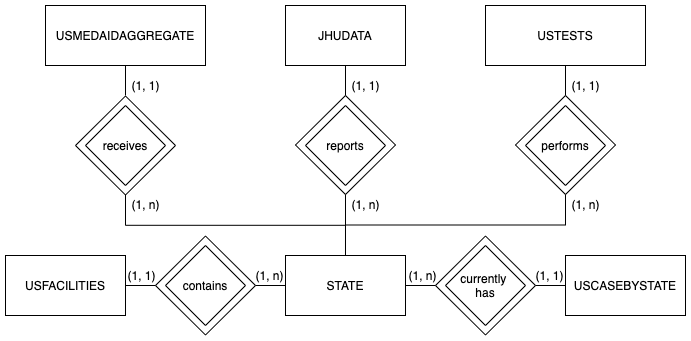
\includegraphics[width=\textwidth]{diagrams/ER2.png}
    \caption{Initial Entity-Relationship Diagram to Model our Data Sources and Relational Database Design}
    \label{fig:er2}
\end{figure}
\FloatBarrier

\pagebreak

\subsection{Database Design}
\label{subsec:design}

\noindent
The database design began with a simple ER diagram, where each data source was assigned a relationship to a parent STATE entity, as shown in Figure \ref{fig:er2}. As will be seen later on, in the actual implementation in section \ref{subsec:implementation}, the data was easily translated to the Third Normal Form (3NF), since the only functional dependency present in the relation was that of the primary key (State, and DateRecorded) determining all other columns (with the exception of the JHUDATA, USFACILITIES, USALLBEDOCCUPANCY, and USICUBEDOCCUPANCY, which are 2NF). However, to reduce the number of NULL values present in the database, the United States Cases By State (USCASEBYSTATE) data source was broken up into several entities (and later translated to several tables), such as recovery, ventilator, hospitalized, and ICU information (with each of those tables only having entries if a state has at least one non-null entry for the day). A similar decomposition was performed for the Aggregated Facility Capacity Count (USFACILITIES) data source into separate ICU bed information and overall bed information. This resulted in a revised ER diagram, seen in Figure \ref{fig:er1}. Finally, this ER diagram was translated to the relational model, and primary and foreign keys were assigned, as seen in Figure \ref{fig:tables}. As can be seen, and later discussed in Section \ref{subsec:implementation}, each of these tables is in fact in Third Normal Form (3NF), such that natural joins result in no spurious tuples and that all of the columns are functionally dependent on solely the primary key. 

\subsubsection{Conceptual Schema}
\label{subsubsec:concept}

\noindent
The conceptual schema for the COVID-19 Database is presented as follows:

\begin{itemize}
    \item Entities and Attributes
    \item Relationships
    \item Final ER Conceptual Schema Diagram (Figure \ref{fig:er1})
    \item Explicit Integrity Constraints
\end{itemize}

\noindent
As is typical, it should be noted that the keys of the entities have been indicated using \textbf{\underline{bold font and a regular underline}}.

\pagebreak

\noindent
\textbf{Entities and Attributes}

\noindent
The entities defined for this databse are: \\

\begin{itemize}
    \item STATE
    \item JHUDATA
    \item USMEDAIDAGGREGATE
    \item USFACILITIES
    \item USICUBEDOCCUPANCY
    \item USALLBEDOCCUPANCY
    \item USCASEBYSTATE
    \item RECOVERED
    \item VENTILATOR
    \item HOSPITALIZED
\end{itemize}

\noindent
A more detailed description of each entity follows:

\begin{description}
\item{\em\bf STATE:} One of the 50 political entities, 5 territories, and the District of Columbia that together make up the U.S. Each state can contain 0, 1,or more national parks (either partially or completely). \\ \\

Some example instances are: New Mexico, New York, California, Georgia. \\
 
\begin{tabular}{llc}
 Attributes: & {\bf \underline{StateAbbreviation}} &  (SSPF) \\
	    & StateName &  (SSPF) \\
\end{tabular} \\
\\

\pagebreak

\item{\em\bf JHUDATA:} John Hopkins Daily COVID-19 Data. \\ \\

An example instance is: JHU Data from Albuquerque, New Mexico for May 10, 2020. \\
 
\begin{tabular}{llc}
 Attributes: & {\bf \underline{DateRecorded} (Month-Day-Year)} &  (CSPF) \\
	    & {\bf \underline{Country}} &  (SSPF) \\
	    & {\bf \underline{State}} & (SSPF) \\
	    & {\bf \underline{City}} & (SSPF) \\
	    & Confirmed & (SSPF) \\
	    & Deaths & (SSPF) \\
	    & Recovered & (SSPF) \\
	    & Active & (SSPF) \\
	    & Latitude & (SSPF) \\
	    & Longitude & (SSPF) \\
\end{tabular} \\
\\

\item{\em\bf USCASEBYSTATE:} Daily COVID-19 Data broken down by State. \\ \\

An example instance is: Number of positive, negative, and total tests performed in New Mexico for May 10, 2020, in addition to the number of deaths and the quality of the data for the day. \\
 
\begin{tabular}{llc}
 Attributes: & {\bf \underline{DateRecorded} (Month-Day-Year)} &  (CSPF) \\
	    & {\bf \underline{State}} &  (SSPF) \\
	    & Positive & (SSPF) \\
	    & Negative & (SSPF) \\
	    & Death & (SSPF) \\
	    & Total & (SSPF) \\
	    & DataQualityGrade & (SSPF) \\
	    & DataGrade & (SSPF) \\
\end{tabular} \\
\\
\textbf{Notes}
\begin{enumerate}
    \item DataQualityGrade: The grade on an A-F scale, of the quality of data provided by the state for a specific day.
    \item DataGrade: The grade on an A-F scale of the data (i.e. how severe is the outbreak in the state) of a state for a specific day.
\end{enumerate} \\

\item{\em\bf HOSPITALIZED:} Number of hospitalizations per state on a daily basis. \\ \\

An example instance is: Number hospitalized patients currently and cumulatively (since the beginning of the pandemic) in New Mexico for May 10, 2020. \\
 
\begin{tabular}{llc}
 Attributes: & {\bf \underline{DateRecorded} (Month-Day-Year)} &  (CSPF) \\
	    & {\bf \underline{State}} &  (SSPF) \\
	    & HospitalizedCurrently & (SSPF) \\
	    & HospitalizedCumulative & (SSPF) \\
\end{tabular} \\

\item{\em\bf ICU:} Number of patients in the ICU per state on a daily basis. \\ \\

An example instance is: Number of ICU patients currently and cumulatively (since the beginning of the pandemic) in New Mexico for May 10, 2020. \\
 
\begin{tabular}{llc}
 Attributes: & {\bf \underline{DateRecorded} (Month-Day-Year)} &  (CSPF) \\
	    & {\bf \underline{State}} &  (SSPF) \\
	    & InICUCurrently & (SSPF) \\
	    & InICUCumulative & (SSPF) \\
\end{tabular} \\

\item{\em\bf VENTIALTOR:} Number of patients on a ventilator per state on a daily basis. \\ \\

An example instance is: Number of patients currently on a ventilator and the number of cumulative patients who have required a ventilator since the beginning of the pandemic in New Mexico for May 10, 2020. \\
 
\begin{tabular}{llc}
 Attributes: & {\bf \underline{DateRecorded} (Month-Day-Year)} &  (CSPF) \\
	    & {\bf \underline{State}} &  (SSPF) \\
	    & OnVentilatorCurrently & (SSPF) \\
	    & OnVentilatorCumulative & (SSPF) \\
\end{tabular} \\

\pagebreak

\item{\em\bf RECOVERED:} Number of recovered COVID-19 patients per state on a daily basis. \\ \\

An example instance is: Number of recovered patients since the beginning of the pandemic in New Mexico for May 10, 2020. \\
 
\begin{tabular}{llc}
 Attributes: & {\bf \underline{DateRecorded} (Month-Day-Year)} &  (CSPF) \\
	    & {\bf \underline{State}} &  (SSPF) \\
	    & Recovered & (SSPF) \\
\end{tabular} \\

\item{\em\bf USFACILITIES:} Population, age distribution, and bed/ICU availability on a per county granularity. \\ \\

An example instance is: Population, demographics, and number of beds in Bernalillo County, New Mexico on May 10, 2020. \\
 
\begin{tabular}{llc}
 Attributes: & {\bf \underline{DateRecorded} (Month-Day-Year)} &  (CSPF) \\
	    & {\bf \underline{State}} &  (SSPF) \\
	    & {\bf \underline{CountyName}} & (SSPF) \\
	    & Population & (SSPF) \\
	    & Population20Plus & (SSPF) \\
	    & Population65Plus & (SSPF) \\
	    & StaffedAllBeds & (SSPF) \\
	    & StaffedICUBeds & (SSPF) \\
	    & LicensedAllBeds & (SSPF) \\
\end{tabular} \\

\item{\em\bf USALLBEDOCCUPANCY:} Current occupancy of hospital beds on a per country granularity. \\ \\

An example instance is: Number between 0 and 1 indicating the level of hospital beds that are occupied in Bernalillo County on May 10, 2020. \\
 
\begin{tabular}{llc}
 Attributes: & {\bf \underline{DateRecorded} (Month-Day-Year)} &  (CSPF) \\
	    & {\bf \underline{State}} &  (SSPF) \\
	    & {\bf \underline{CountyName}} & (SSPF) \\
	    & AllBedOccupancyRate & (SSPF) \\
\end{tabular} \\

\item{\em\bf USICUBEDOCCUPANCY:} Current occupancy of ICU beds/units on a per country granularity. \\ \\

An example instance is: Number between 0 and 1 indicating the level of ICU beds/units that are occupied in Bernalillo County on May 10, 2020. \\
 
\begin{tabular}{llc}
 Attributes: & {\bf \underline{DateRecorded} (Month-Day-Year)} &  (CSPF) \\
	    & {\bf \underline{State}} &  (SSPF) \\
	    & {\bf \underline{CountyName}} & (SSPF) \\
	    & ICUBedOccupancyRate & (SSPF) \\
\end{tabular} \\

\item{\em\bf USMEDAIDAGGREGATE:} Cumulative amount of medical aid sent to a state since the start of the pandemic. Includes number of packages, cost of material, and weight of received packages. \\ \\

An example instance is: Cumulative number of packages, the cost of the packages, and the weight of the packages received by New Mexico up to May 10, 2020. \\
 
\begin{tabular}{llc}
 Attributes: & {\bf \underline{DateRecorded} (Month-Day-Year)} &  (CSPF) \\
	    & {\bf \underline{State}} &  (SSPF) \\
	    & Deliveries & (SSPF) \\
	    & Cost & (SSPF) \\
	    & Weight & (SSPF) \\
\end{tabular} \\
\end{description}
\pagebreak

\noindent
\textbf{Relationships}

\noindent
The relationships in this schema are listed and described below. \\

\begin{description}
\item [tests]

\noindent
A state performs COVID-19 tests, each of which may be positive or negative. This relationship keeps track of the daily tests in the United States and their associated data.

\begin{tabular}{lllc}  
  Attributes: None \\
\end{tabular}

\item [receives]

\noindent
A state receives medical aid from industry or the federal government. This relationship keeps track of the aid received by states in terms of the cost of the aid, the number of received packages, and the weight of the received packages.

\begin{tabular}{lllc}
     Attributes: None \\
\end{tabular}

%\item [performs]

%\noindent
%The United States performs tests in each state every day. This relationship keeps track of the aggregate number of tests performed everyday, and from where the tests are coming from (a CDC lab or a Public Health lab)

%\begin{tabular}{lllc}
%     Attributes: None \\
%\end{tabular}

\item [contains]

\noindent
A state contains facilities, such as hospitals, beds, and ICU units. This relationship keeps track of the number of these available to each state, and the current occupancy level of the available facilities.

\begin{tabular}{lllc}
    Attributes: None \\
\end{tabular}

\item [provides]

\noindent
A facility provides a certain number of ICU units, and each facility has a certain occupancy rate of those units. This relationship keeps track of the occupancy rate and availability of those ICU units.

\begin{tabular}{lllc}
     Attributes: None \\
\end{tabular}

\item [supplies]

\noindent
A facility also supplies a certain number of staffed beds. This relationship keeps track of how many beds a facility provides and how many beds a facility is currently using (as a rate).

\begin{tabular}{lllc}
    Attributes: None \\
\end{tabular}

\item [currentlyHas]

\noindent
Each state currently has a certain number of COVID-19 cases. This relationship keeps track of those cases by state, in addition to allowing the information from them child relationship and entities, such as recovered patients, patients in the ICU, patients on ventilators, and hospitalized patients, to propagate upwards and be associated with particular states.

\begin{tabular}{lllc}
    Attributes: None \\
\end{tabular}

\item [patients]

\noindent
Each set of cases has a number of recovered patients, which this relationship keeps track of daily.

\begin{tabular}{lllc}
    Attributes: None \\
\end{tabular}

\item [connectTo]

\noindent
Each set of cases in a state has a number of patients connected to ventilators. This relationship keeps track of that statistic at the state-wide level on a daily basis.

\begin{tabular}{lllc}
    Attributes: None \\
\end{tabular}

\item [occupied]

\noindent
Each set of cases in a state has a count of the number of patients that are currently occupying ICU units. This relationship keeps track of and updates that statistic daily.

\begin{tabular}{lllc}
    Attributes: None \\
\end{tabular}

\item [checkedIn]

\noindent
Each set of cases in a state has a current count of the number of hospitalized COVID-19 patients, and this relationship tracks that daily.

\begin{tabular}{lllc}
    Attributes: None \\
\end{tabular}

\end{description}

\noindent
\textbf{Explicit Integrity Constraints} \\

\noindent
Some examples of integrity constrains in our COVID-19 database follow:

\begin{enumerate}
    \item In the STATE entity, there should be exactly 59 entries (50 states, 5 territories and DC, and the Diamond Princess, Grand Princess, and Recovered) in order to accommodate the data from the API.
    \item The USCASEBYSTATE entity should have 56 new entries for each day it is updated (one for each of the 50 states, 5 territories and DC). For example, if data collection has been occurring for 6 days, there should be exactly 336 entries.
    \item The USCASEBYSTATE entity must have consistency, such that the number of recovered patients + the number of deaths + the number of positive cases + the number of negative cases = the total number of tests.
\end{enumerate}

\pagebreak

\noindent
\textbf{Final ER Conceptual Schema Diagram}

\FloatBarrier
\begin{figure}[h]
    \centering
    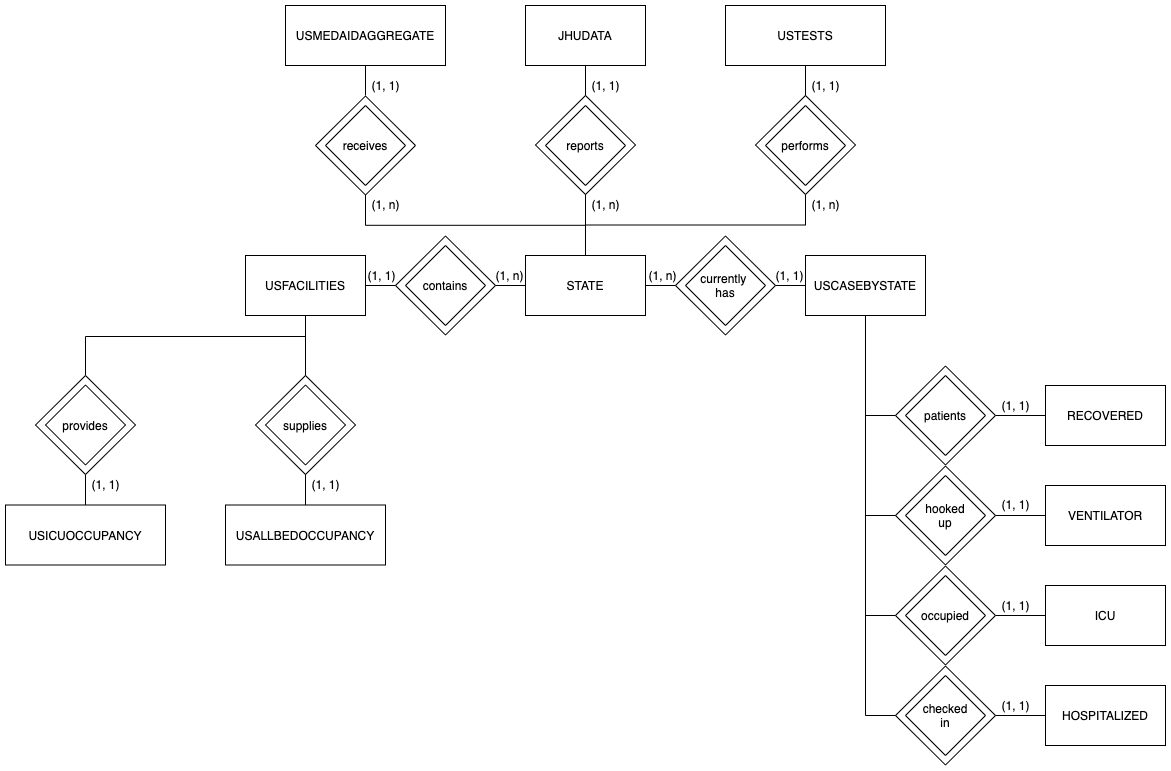
\includegraphics[width=\textwidth]{diagrams/ER1.png}
    \caption{Basic Entity-Relationship Diagram to Model our Data Sources and Relational Database Design}
    \label{fig:er1}
\end{figure}
\FloatBarrier

\pagebreak

\subsection{Database Implementation}
\label{subsec:implementation}

\noindent
The database was constructed by translating the final ER Diagram in Figure \ref{fig:er1} to the relational model, as seen on the next page in Figure \ref{fig:tables}. A SQL script was then written (CreateDB.sql) to implement the schema in the Oracle Cloud DBMS, and the database was then used to collect data to provide the ability to perform useful queries that aided in the analysis presented in Section \ref{sec:analysis}.

\noindent
Note that every table in the relational database shown in Figure \ref{fig:tables} is in fact in 3NF, except for the JHUDATA, USFACILITIES (and its children USALLBEDOCCUPANCY and USICUBEDOCCUPANCY) tables (the JHUDATA table was not further normalized or decomposed as it seemed unnecessary since we are solely focusing on US data and an additional CITY and/or COUNTRY tables would have been unneeded - the same can be said for the other tables since CountyName proved to be unneeded for our purposes). For the STATE table, the StateName is functionally dependent solely on the StateAbbreviation private key, while for the remaining tables, their columns are functionally dependent solely on the primary key of DateRecorded and State.

\noindent
Also note that DateRecorded was an added column to the raw data to allow for the storage of a snapshot of the state of the COVID-19 pandemic in the United States on each day. This provided the time series capability of the database, and resulted in the peculiar property that each tuple once entered, is not modified such that the database only continues to grow each day as new entries for the day are entered (i.e. only INSERT operations and no UPDATE operations).

\begin{figure}[H]
\begin{adjustwidth*}{}{-4em}
\resizebox{1.5\textwidth}{!}{%
\begin{tikzpicture}[relation/.style={rectangle split, rectangle split parts=#1, rectangle split part align=base, draw, anchor=center, align=center, text height=3mm, text centered}]\hspace*{-0.5cm}

% RELATIONS

\node (statetitle) {\textbf{STATE}};

\node [relation=2, rectangle split horizontal, rectangle split part fill={lightgray!50}, anchor=north west, below=0.6cm of statetitle.west, anchor=west] (state)
{\underline{StateAbbreviation}%
\nodepart{two}   StateName};

\node [below=1.3cm of state.west, anchor=west] (jhutitle) {\textbf{JHUDATA}};

\node [relation=10, rectangle split horizontal, rectangle split part fill={lightgray!50}, below=0.6cm of jhutitle.west, anchor=west] (jhu)
{\underline{DateRecorded}%
\nodepart{two} \underline{Country}
\nodepart{three} \underline{State}
\nodepart{four}  \underline{City}
\nodepart{five}  Confirmed
\nodepart{six} Deaths
\nodepart{seven} Recovered
\nodepart{eight} Active
\nodepart{nine} Latitude
\nodepart{ten} Longitude};

\node [below=1.3cm of jhu.west, anchor=west] (uscasetitle) {\textbf{USCASEBYSTATE}};

\node [relation=8, rectangle split horizontal, rectangle split part fill={lightgray!50}, below=0.6cm of uscasetitle.west, anchor=west] (uscase)
{\underline{DateRecorded}%
\nodepart{two} \underline{State}
\nodepart{three} Positive
\nodepart{four}  Negative
\nodepart{five}  Death
\nodepart{six} Total
\nodepart{seven} DataQualityGrade
\nodepart{eight} DataGrade};

\node [below=1.3cm of uscase.west, anchor=west] (hospitalizedtitle) {\textbf{HOSPITALIZED}};

\node [relation=4, rectangle split horizontal, rectangle split part fill={lightgray!50}, below=0.6cm of hospitalizedtitle.west, anchor=west] (hospitalized)
{\underline{DateRecorded}%
\nodepart{two} \underline{State}
\nodepart{three} HospitalizedCurrently
\nodepart{four}  HospitalizedCumulative};

\node [below=1.3cm of hospitalized.west, anchor=west] (icutitle) {\textbf{ICU}};

\node [relation=4, rectangle split horizontal, rectangle split part fill={lightgray!50}, below=0.6cm of icutitle.west, anchor=west] (icu)
{\underline{DateRecorded}%
\nodepart{two} \underline{State}
\nodepart{three} InICUCurrently
\nodepart{four}  InICUCumulative};
  
\node [below=1.3cm of icu.west, anchor=west] (ventilatortitle) {\textbf{VENTILATOR}};

\node [relation=4, rectangle split horizontal, rectangle split part fill={lightgray!50}, below=0.6cm of ventilatortitle.west, anchor=west] (ventilator)
{\underline{DateRecorded}%
\nodepart{two} \underline{State}
\nodepart{three} OnVentilatorCurrently
\nodepart{four}  OnVentilatorCumulative};
  
\node [below=1.3cm of ventilator.west, anchor=west] (recoveredtitle) {\textbf{RECOVERED}};

\node [relation=3, rectangle split horizontal, rectangle split part fill={lightgray!50}, below=0.6cm of recoveredtitle.west, anchor=west] (recovered)
{\underline{DateRecorded}%
\nodepart{two} \underline{State}
\nodepart{three} Recovered};

\node [below=1.3cm of recovered.west, anchor=west] (facilitytitle) {\textbf{USFACILITIES}};

\node [relation=9, rectangle split horizontal, rectangle split part fill={lightgray!50}, below=0.6cm of facilitytitle.west, anchor=west] (facility)
{\underline{DateRecorded}%
\nodepart{two} \underline{State}
\nodepart{three} \underline{CountyName}
\nodepart{four} Population
\nodepart{five} Population20Plus
\nodepart{six} Population65Plus
\nodepart{seven} StaffedAllBeds
\nodepart{eight} StaffedICUBeds
\nodepart{nine} LicensedAllBeds};

\node [below=1.3cm of facility.west, anchor=west] (allbedtitle) {\textbf{USALLBEDOCCUPANCY}};

\node [relation=4, rectangle split horizontal, rectangle split part fill={lightgray!50}, below=0.6cm of allbedtitle.west, anchor=west] (allbed)
{\underline{DateRecorded}%
\nodepart{two} \underline{State}
\nodepart{three} \underline{CountyName}
\nodepart{four} AllBedOccupancyRate};
  
\node [below=1.3cm of allbed.west, anchor=west] (icubedtitle) {\textbf{USICUBEDOCCUPANCY}};

\node [relation=4, rectangle split horizontal, rectangle split part fill={lightgray!50}, below=0.6cm of icubedtitle.west, anchor=west] (icubed)
{\underline{DateRecorded}%
\nodepart{two} \underline{State}
\nodepart{three} \underline{CountyName}
\nodepart{four} ICUBedOccupancyRate};

\node [below=1.3cm of icubed.west, anchor=west] (medaidtitle) {\textbf{USMEDAIDAGGREGATE}};

\node [relation=5, rectangle split horizontal, rectangle split part fill={lightgray!50}, below=0.6cm of medaidtitle.west, anchor=west] (medaid)
{\underline{DateRecorded}%
\nodepart{two} \underline{State}
\nodepart{three} Deliveries
\nodepart{four} Cost
\nodepart{five} Weight};

%\node [below=1.3cm of medaid.west, anchor=west] (testtitle) {\textbf{USTESTS}};

%\node [relation=4, rectangle split horizontal, rectangle split part fill={lightgray!50}, below=0.6cm of testtitle.west, anchor=west] (test)
%{\underline{DateRecorded}%
%\nodepart{two} \underline{DateCollected}
%\nodepart{three} CDCLabs
%\nodepart{four} USPublicHealthLabs};


  
% FOREIGN KEYS

\draw[-latex] (jhu.three south) -- ++(0,-0.3) -| ($(jhu.one south) + (-2,0)$) |- ($(state.one south) + (0.25,-0.50)$) -| ($(state.one south) + (0.25,0)$);

\draw[-latex] (uscase.two south) -- ++(0,-0.3) -| ($(uscase.one south) + (-2,0)$) |- ($(state.one south) + (0.25,-0.50)$) -| ($(state.one south) + (0.25,0)$);

\draw[-latex] (hospitalized.one south) -- ++(0,-0.3) -| ($(hospitalized.one south) + (-2,0)$) |- ($(uscase.one south) + (0.25,-0.50)$) -| ($(uscase.one south) + (0.25,0)$);

\draw[-latex] (hospitalized.two south) --++(0, -0.3) -| ($(hospitalized.one south) + (-2,0)$) |- ($(uscase.one south) + (0.25,-0.50)$) -| ($(uscase.two south) + (0.25,0)$);

\draw[-latex] (icu.one south) -- ++(0,-0.3) -| ($(icu.one south) + (-2,0)$) |- ($(uscase.one south) + (0.25,-0.50)$) -| ($(uscase.one south) + (0.25,0)$);

\draw[-latex] (icu.two south) --++(0, -0.3) -| ($(icu.one south) + (-2,0)$) |- ($(uscase.one south) + (0.25,-0.50)$) -| ($(uscase.two south) + (0.25,0)$);

\draw[-latex] (ventilator.one south) -- ++(0,-0.3) -| ($(ventilator.one south) + (-2,0)$) |- ($(uscase.one south) + (0.25,-0.50)$) -| ($(uscase.one south) + (0.25,0)$);

\draw[-latex] (ventilator.two south) --++(0, -0.3) -| ($(ventilator.one south) + (-2,0)$) |- ($(uscase.one south) + (0.25,-0.50)$) -| ($(uscase.two south) + (0.25,0)$);

\draw[-latex] (recovered.one south) -- ++(0,-0.3) -| ($(recovered.one south) + (-2,0)$) |- ($(uscase.one south) + (0.25,-0.50)$) -| ($(uscase.one south) + (0.25,0)$);

\draw[-latex] (recovered.two south) --++(0, -0.3) -| ($(recovered.one south) + (-2,0)$) |- ($(uscase.one south) + (0.25,-0.50)$) -| ($(uscase.two south) + (0.25,0)$);

\draw[-latex] (facility.two south) -- ++(0,-0.3) -| ($(facility.one south) + (-3,0)$) |- ($(state.one south) + (0.25,-0.50)$) -| ($(state.one south) + (0.25,0)$);

\draw[-latex] (allbed.one south) -- ++(0,-0.3) -| ($(allbed.one south) + (-2,0)$) |- ($(facility.one south) + (0.25,-0.50)$) -| ($(facility.one south) + (0.25,0)$);

\draw[-latex] (allbed.two south) --++(0, -0.3) -| ($(allbed.one south) + (-2,0)$) |- ($(facility.one south) + (0.25,-0.50)$) -| ($(facility.two south) + (0.25,0)$);

\draw[-latex] (allbed.three south) --++(0, -0.3) -| ($(allbed.one south) + (-2,0)$) |- ($(facility.one south) + (0.25,-0.50)$) -| ($(facility.three south) + (0.25,0)$);

\draw[-latex] (icubed.one south) -- ++(0,-0.3) -| ($(icubed.one south) + (-2,0)$) |- ($(facility.one south) + (0.25,-0.50)$) -| ($(facility.one south) + (0.25,0)$);

\draw[-latex] (icubed.two south) --++(0, -0.3) -| ($(icubed.one south) + (-2,0)$) |- ($(facility.one south) + (0.25,-0.50)$) -| ($(facility.two south) + (0.25,0)$);

\draw[-latex] (icubed.three south) --++(0, -0.3) -| ($(icubed.one south) + (-2,0)$) |- ($(facility.one south) + (0.25,-0.50)$) -| ($(facility.three south) + (0.25,0)$);

\draw[-latex] (medaid.two south) -- ++(0,-0.3) -| ($(medaid.one south) + (-3,0)$) |- ($(state.one south) + (0.25,-0.50)$) -| ($(state.one south) + (0.25,0)$);

\end{tikzpicture}
}%
\end{adjustwidth*}
\caption{COVID-19 Relational Schema}
\label{fig:tables}
\end{figure}	

\subsection{Data Insertion and Extraction for Analysis}
\label{subsec:insertextract}

\noindent
The data was collected between 5 MST and 7 MST everyday from May 6, 2020 until May 13, 2020 using the \MYhref{https://www.npmjs.com/package/covid19-api}{Covid-19 API} and a python script (GatherData.py). This process involved posting a GET request to the 5 endpoints described in Section \ref{subsec:sourcedata} and obtaining the data in JSON format. 

\noindent
Since some of the data included irrelevant and extraneous columns, the python script first removed those extra columns and converted the data to CSV format to begin prepping for upload to our database instance on Oracle Cloud. Next, since the data needed to be broken down into a file for each of the 11 tables (excluding that STATE table), the python script organized the data into 11 files, taking care that the columns of each CSV file corresponded with the columns of each table in the instance of the database.

\noindent
This allowed the users to run the python script once every evening to collect and organize data, and subsequently upload the data into Oracle Cloud. Backups of the raw data obtained from the COVID-19 API endpoints, in addition to backups of the processed data. This process and the results of the analyses from the data entered and extracted from the database is covered in Section \ref{sec:analysis}. An overview of this process can be found in Figures \ref{fig:my_label} - \ref{fig:tbl_bd}.

\FloatBarrier
\begin{figure}[h]
    \centering
    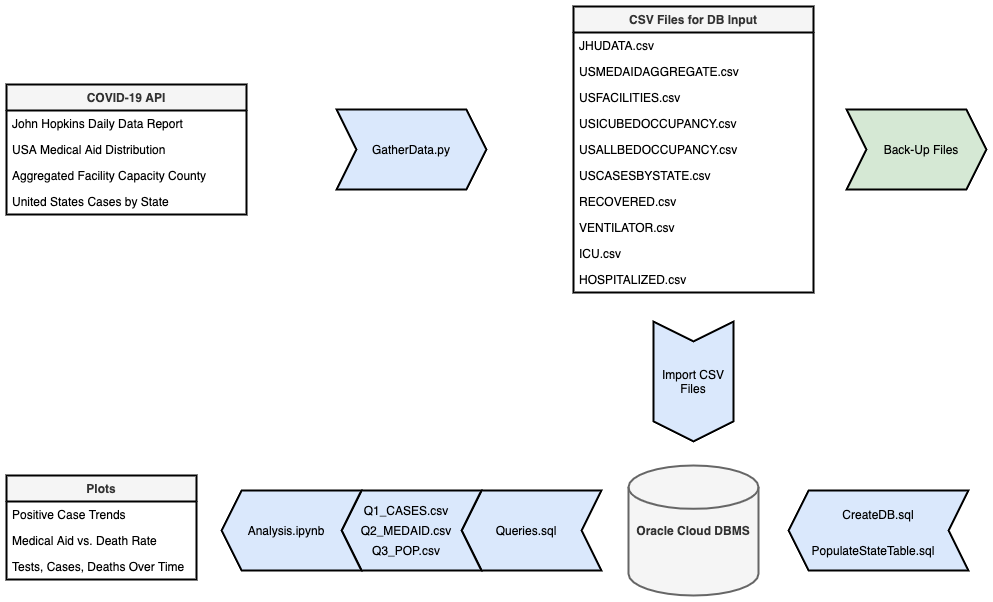
\includegraphics[width=\textwidth]{diagrams/DataInsertionExtraction.png}
    \caption{Data Insertion and Extraction Workflow Overview}
    \label{fig:my_label}
\end{figure}
\FloatBarrier

\pagebreak

\section{Data Analysis}
\label{sec:analysis}

\noindent
We performed a number of analyses to demonstrate the viability of our design and collected data for the kind of analyses that both experts and enthusiasts might be interested in performing. We mainly used SQL queries and Python's data science toolset (Pandas\cite{citepandas}, NumPy\cite{citenumpy}, ScikitLearn\cite{cite_scikit-learn}) to retrieve, prepare, and analyze our data. The following sections provides details on our approach in preparing the data and performing the analysis.

\subsection{Data Preparation}

\noindent
We divided the large tuples of raw data retrieved from our sources into multiple tables (Figure \ref{fig:tbl_bd}). In addition to resulting in a much more logical representation, this approach resulted in far fewer NULL values in the table. The Python script to retrieve and divide the data resides in the GatherData.py file.

\FloatBarrier
\begin{figure}[h]
    \centering
    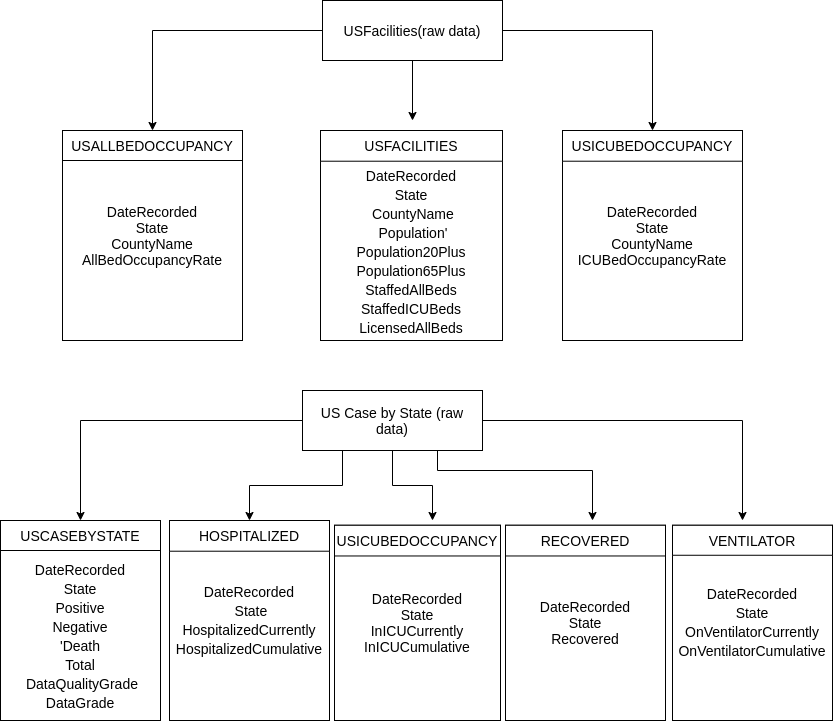
\includegraphics[width=0.8\textwidth]{diagrams/data_breakdown.png}
    \caption{Breaking down the raw data into multiple tables. Note that the arrows simply represent the flow of data and do not connote any database design related concept}
    \label{fig:tbl_bd}
\end{figure}
\FloatBarrier

\noindent
We explored the following items in the data:
\begin{itemize}
    \item Trends in tests, positive and negative cases, and deaths at the State Level
    \item Correlation of tests with medical aid at the state level
    \item Hospital resources as a predictor of death rate
\end{itemize}
In order to perform these analyses, we used simple SQL queries against our database to retrieve the data and simple python scripts to analyze the data and visualize the results. The queries used to retrieve the historic data from our database can be found in the `Queries' folder and the Python scripts for analyzing and visualizing the data can be found in the `analysis.ipynb' Jupyter Notebook.

\pagebreak

\subsection{Tests, Cases, and Deaths at the State Level}
\label{subsec:StateLevel}

\noindent
Figure \ref{fig:pos_trends} shows the number of positive cases in four states and the predictions projected two days into the feature using regression analysis.
\subsubsection{Approach}
We used the `USTESTBYSTATES' table to retrieve historical trends for the states. The result of the query was exported to a \textit{csv} file and imported into the python script for plotting and regression analysis.

\FloatBarrier
\begin{figure}[h]
     \centering
     \begin{subfigure}[b]{0.49\textwidth}
         \centering
         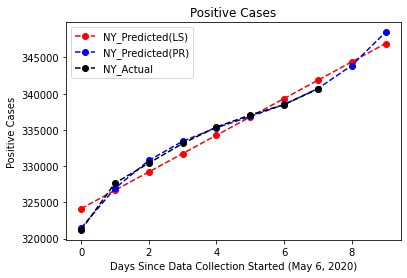
\includegraphics[width=\textwidth]{diagrams/analysis/positive_trend_NY.png}
         \caption{Positive cases trends for NY}
     \end{subfigure}
     \begin{subfigure}[b]{0.49\textwidth}
         \centering
         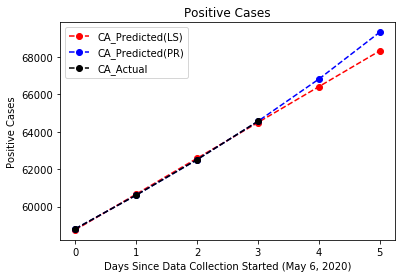
\includegraphics[width=\textwidth]{diagrams/analysis/positive_trend_CA.png}
         \caption{Positive cases trends for CA}
     \end{subfigure}
        \label{fig:three graphs}
             \begin{subfigure}[b]{0.49\textwidth}
         \centering
         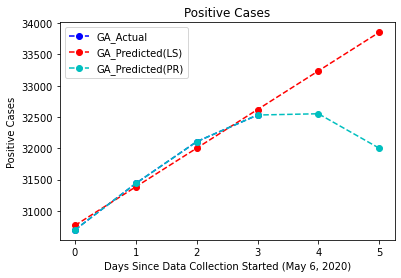
\includegraphics[width=\textwidth]{diagrams/analysis/positive_trend_GA.png}
         \caption{Positive cases trends for GA}
     \end{subfigure}
     \begin{subfigure}[b]{0.49\textwidth}
         \centering
         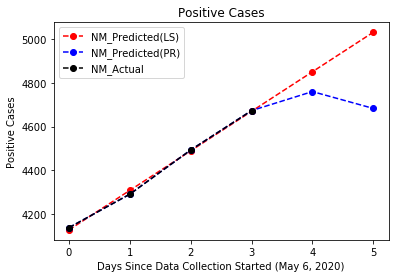
\includegraphics[width=\textwidth]{diagrams/analysis/positive_trend_NM.png}
         \caption{Positive cases trends for NM}
         \label{fig:three sin x}
     \end{subfigure}
        \caption{The number of positive cases for CA, GA, NY, NM and predictions for two days into the future using linear(LS) and polynomial regression (PR3)}
        \label{fig:pos_trends}

\end{figure}
\FloatBarrier

\noindent
The SQL command used to obtain this data is presented below:
\begin{lstlisting}[language=SQL,
        deletekeywords={IDENTITY,INT},
        morekeywords={clustered},    
        framesep=10pt,
        framextopmargin=10pt]
    SELECT DateRecorded, State, Positive, Negative, Total, Death 
    FROM USCASEBYSTATE
    ORDER BY State;\end{lstlisting}
    
\pagebreak

\subsection{Correlation of Tests with Medical Aid at the State Level}
\noindent
We looked the historical test and medical aid data in our database to look for the relationship between the amount of medical aid a state receives and the number of tests the state performs. 

\subsubsection{Approach}
We joined two tables `USCASEBYSTATE' and `USMEDAIDAGGREGATE', on the timestamp and state attributes and returned the total monetary value of the aid received and the number of tests performed. 

%\FloatBarrier
%\begin{figure}[h]
%    \centering
%    
\includegraphics[scale=0.5]{diagrams/analysis/medaid_corr_no_outliers.png}
%    \caption{Number of tests conducted vs the amount of medical aid received by states with a line fit through the data using least squares}
%    \label{fig:test_cost_fit}
%\end{figure}
%\FloatBarrier

%\FloatBarrier
%\begin{figure}[h]
%    \centering
%    
\includegraphics[scale=0.5]{diagrams/analysis/medaid_corr_outliers.png}
%    \caption{Number of tests conducted vs the amount of medical aid received by states with a line fit through the data using least squares}
%    \label{fig:test_cost_fit}
%\end{figure}
%\FloatBarrier

\FloatBarrier
\begin{figure}[h]
    \centering
    \begin{subfigure}[h]{0.5\textwidth}
        \centering
        
\includegraphics[width=\linewidth]{diagrams/analysis/medaid_corr_no_outliers.png}
        \caption{Without outliers.}
        \label{fig:test_cost_fit}
    \end{subfigure}%
    \begin{subfigure}[h]{0.5\textwidth}
        \centering
        
\includegraphics[width=\linewidth]{diagrams/analysis/medaid_corr_outliers.png}
        \caption{With outliers.}
    \end{subfigure}
    \label{fig:test_cost_fit}
    \caption{Number of tests conducted vs the amount of medical aid received by states (for all 50 states, 5 territories, and DC) with a line fit through the data using least squares.}
\end{figure}
\FloatBarrier

\noindent
The SQL command used to obtain this data is presented below:
\begin{lstlisting}[language=SQL,
        deletekeywords={IDENTITY,INT},
        morekeywords={clustered},    
        framesep=10pt,
        framextopmargin=10pt]
    SELECT u.DateRecorded, u.State, u.Positive, u.Negative, u.Total AS test_total, u.Death, ma.Deliveries, ma.Cost, ma.Weight
    FROM USCASEBYSTATE u, USMEDAIDAGGREGATE ma
    WHERE u.State = ma.State AND u.DateRecorded = ma.DateRecorded 
    ORDER BY u.State, u.DateRecorded;\end{lstlisting}
\pagebreak

\subsection{Hospital Resources as a Predictor of Cases and Deaths}

\noindent
In order to demonstrate the viability of our database for more ambitious analyses, we decided to look at the occupancy rate of ICUs and the number of deaths per capita. 

\subsubsection{Approach}
We performed a 3-way join on JHUDATA, USICUBEDOCCUPANCY, and USFACILITIES and performed some aggregate operations to obtain the average ICU occupancy rate and total number of fatalities and the population for each state. We normalized the total number of fatalities and plotted them as shown in Figure \ref{fig:death_pop_icu}.

\FloatBarrier
\begin{figure}[h]
    \centering
    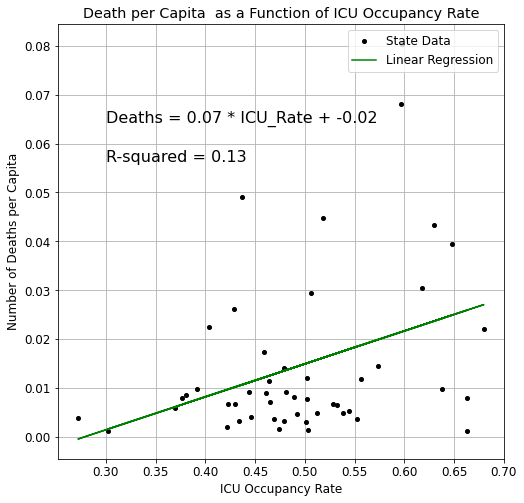
\includegraphics[width=0.65\linewidth]{diagrams/analysis/death_icu.png}
    \caption{The rate of death per capita vs the ICU occupancy rate (of all 50 states, 5 territories, and DC) with a line fit through the data using least squares}
    \label{fig:death_pop_icu}
\end{figure}
\FloatBarrier

\noindent
Obviously, according to Figure \ref{fig:death_pop_icu}, there does not seem to be a strong correlation between ICU occupancy rate (as reported) and the number of deaths per capita. However, there are always issues of whether the reported data is accurate, and there are many other variables that could influence the death rate in specific regions.
\pagebreak

\noindent
The SQL command used to obtain this data is presented below:
\begin{lstlisting}[language=SQL,
        deletekeywords={IDENTITY,INT},
        morekeywords={clustered},    
        framesep=10pt,
        framextopmargin=10pt]
    SELECT f.State, f.DateRecorded, total_pop, icu_avg, j.death_tot 
    FROM(
        SELECT f.State, f.DateRecorded, sum(Population) AS total_pop 
        FROM USFACILITIES f 
        WHERE  DateRecorded=to_date('05/09/2020','MM/DD/YYYY')  
        GROUP BY State, DateRecorded
        ) f , 
        (SELECT o.State, o.DateRecorded, round(avg(ICUBedOccupancyRate),3) AS     icu_avg 
        FROM USICUBEDOCCUPANCY o 
        WHERE o.DateRecorded=to_date('05/09/2020','MM/DD/YYYY')  
        GROUP BY o.State, DateRecorded
        ) o, 
        (SELECT sum(Deaths) AS death_tot, j.State, j.DateRecorded 
        FROM JHUDATA j 
        WHERE DateRecorded=to_date('05/09/2020','MM/DD/YYYY')   
        GROUP BY State, DateRecorded) j 
    WHERE f.State=o.State AND j.State=o.State;\end{lstlisting}

\pagebreak

\section{Conclusions}
In this work we designed a database for keeping a history of COVID-19 data. We demonstrated that our design is able to incorporate and store data from multiple sources and present them in a logical and practical fashion. Adding the timestamps and using natural identifiers, such as the state names, for the records allowed us to easily combine the data gathered from different sources and use them in our sample analyses. These sample analyses showed that our design and the data we collect allow for statistical studies to unveil COVID-19 related trends and correlations. If in order to perform a new analysis, it becomes necessary to incorporate new sources into the database, the new data can be easily integrated into our design to be used in conjunction with the existing data.\\

\noindent
As we planned and executed different phases of this project, we realized that the most involved and sensitive part of the project was designing the database. In other words, once a good database design was achieved and the data was stores properly, retrieving the data and performing analyses on it was fairly straightforward.\\

\noindent
 A common question regarding COVID-19 is that whether or not the temperature has a meaningful impact on the spread of the disease. Hence an interesting possible extension for this work is finding a reliable source of weather information and combining that with the existing mortality and disease progression data. A careful researcher can use our data to potentially study the impact of temperature on the spread of the virus while normalizing for other factors.

%\section{Future Work}
\bibliographystyle{acm}
\bibliography{refs.bib}

\appendix

\section{Other Analyses and Visualizations}

\noindent
Lastly, we provide a few visualizations of the progression of the COVID-19 pandemic from May 6, 2020 - May 13, 2020 with the charts below. The data required for the visualizations below was obtained with the same SQL command as was used in section \ref{subsec:StateLevel}.

\FloatBarrier
\begin{figure}[h]
    \centering
    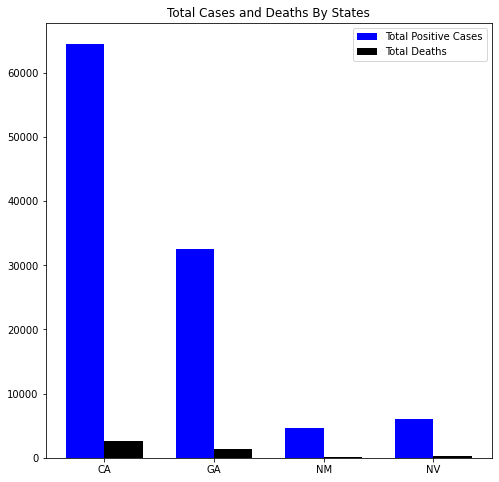
\includegraphics[width=\linewidth]{diagrams/analysis/total_cases_bar.png}
    \caption{Total Cases and Deaths in California, Georgia, New Mexico, Nevada, and New York, as of May 13, 2020.}
    \label{fig:overall}
\end{figure}
\FloatBarrier

\FloatBarrier
\begin{figure}[h]
    \centering
    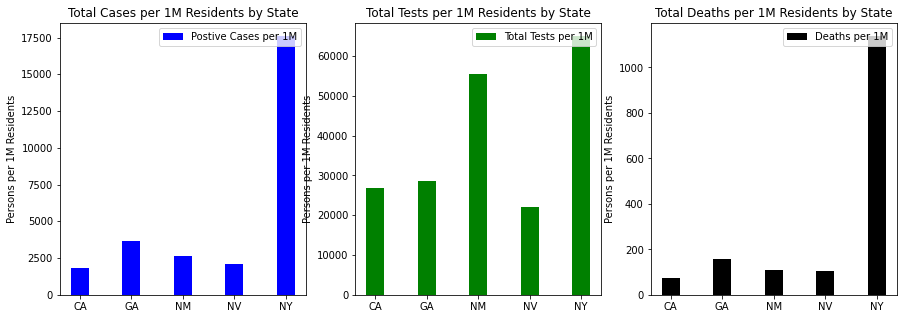
\includegraphics[width=\linewidth]{diagrams/analysis/total_cases_capita_bar.png}
    \caption{Cases and Deaths per 1 million residents in California, Georgia, New Mexico, Nevada, and New York, as of May 13, 2020.}
    \label{fig:capita}
\end{figure}
\FloatBarrier

\noindent
As can be seen in Figure \ref{fig:overall}, by the raw values, New York is performing the most tests, has the most cases, and has the most deaths by a large margin (California has performed a similar number of tests). However, once normalized by population (Figure \ref{fig:capita}, we see that New Mexico is also performing a substantial number of tests per capita, while Georgia has the second most cases and deaths per capita of the 5 states, behind New York.

\pagebreak

\FloatBarrier
\begin{figure}[h]
    \centering
    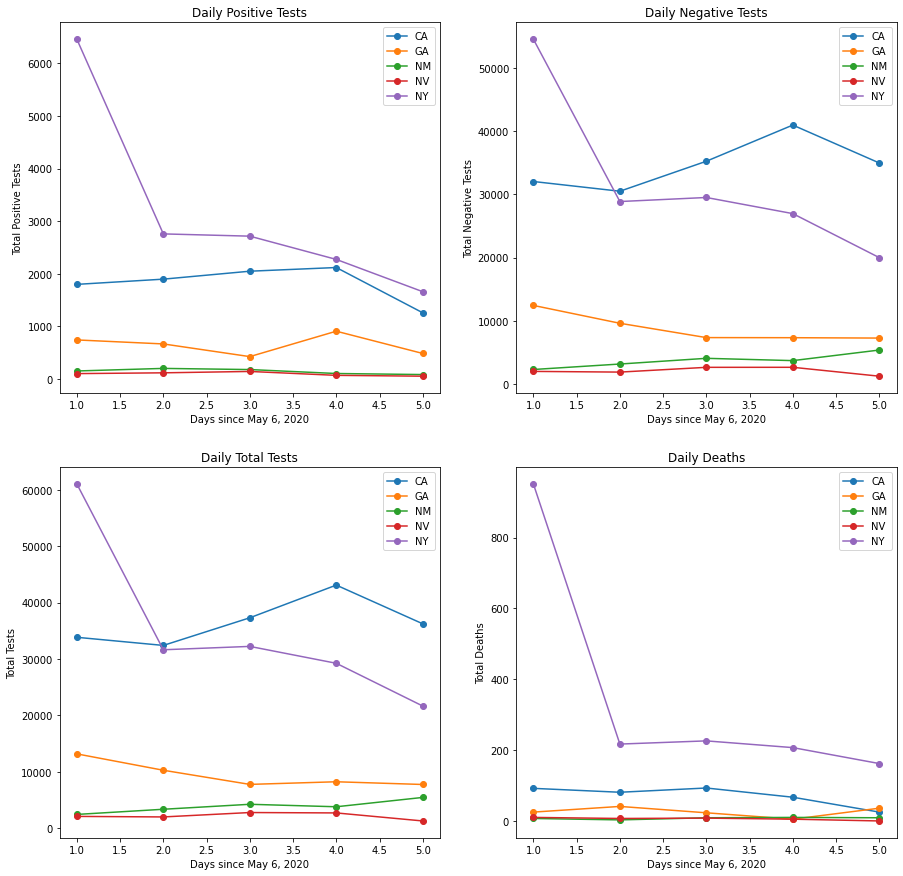
\includegraphics[width=\linewidth]{diagrams/analysis/daily_tests.png}
    \caption{Daily Tests from May 6 - May 13 in California, Georgia, New Mexico, Nevada, and New York.}
    \label{fig:dailytests}
\end{figure}
\FloatBarrier

\noindent
As can be seen in Figure \ref{fig:dailytests}, it is apparent that New York is on the down slope, as their number of positive tests and deaths continues to decrease. However, due to only gathering data for a week and knowing that the data reports have a weekly oscillation (typically peaks on Tuesday and is low Saturday-Monday), it is hard to draw many conclusions from only a week of data that we have been able to gather.

\pagebreak

\FloatBarrier
\begin{figure}[h]
    \centering
    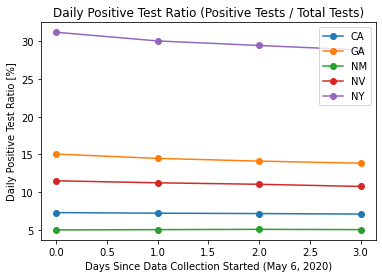
\includegraphics[width=\linewidth]{diagrams/analysis/percent_positive.png}
    \caption{Daily Positive Test Ratio from May 6 - May 13 in California, Georgia, New Mexico, Nevada, and New York.}
    \label{fig:percentpositive}
\end{figure}
\FloatBarrier

\noindent
As can be seen in Figure \ref{fig:percentpositive}, as the volume of testing continues to increase and more people continue to stay at home, the daily positive testing ratio continues to decrease across all 5 states, with New York having the worst ratio and New Mexico having the best ratio. \\

\noindent
The code used to generate these plots can be found in Analysis.ipynb.

%\section{Original Data From EndPoints}

%\noindent
%JHU CSV Columns :
%\comment{filter on country==us; keep villages, state is foreign key to other tables}:

%\begin{itemize}
%    \item Active
%    \item Combined\_Key
%    \item Confirmed
%    \item Country\_Region
%    \item Deaths
%    \item Last\_Update
%    \item Lat
%    \item Long\_
%    \item Province\_State
%    \item Recovered
%\end{itemize}

%\noindent
%Tests in US CSV Columns (1 Entry for every day since January 18, 2020):
%\comment{own table}:

%\begin{itemize}
%    \item CDC Labs
%    \item DateCollected
%    \item USPublicHealthLabs
%\end{itemize}

%\noindent
%USCasesByState CSV Columns:

%\begin{itemize}
%    \item checkTimeEt
%    \item commercialScore
%    \item dataGrade
%    \item dataQualityGrade
%    \item dateChecked
%    \item dataModified
%    \item death
%    \item fips
%    \item hospitalized
%    \item hospitalizedCumulative
%    \item hospitalizedCurrently
%    \item inIcuCumulative
%    \item inIcuCurrently
%    \item lastUpdateEt
%    \item negative
%    \item negativeRegularScore
%    \item negavtiveScore
%    \item onVentilatorCumulative
%    \item onVentilatorCurrently
%    \item pending
%    \item positive
%    \item positiveScore
%    \item posNeg
%    \item recovered
%    \item score
%    \item state
%    \item total
%    \item totalTestResults
%\end{itemize}


%\noindent
%(Not doing this one) FatalityAge CSV Columns:

%\begin{itemize}
%    \item 3 (Number of Deaths)
%    \item 4 (Without Underlying Conditions)
%    \item 5 (Unknown if with Underlying Conditions)
%    \item 6 (Share of Deaths of Unknown + w/o Conditions)
%    \item Age
%    \item DeathRateAllCases (Share of Deaths)
%    \item DeathRateConfirmed (Number of Deaths)
%\end{itemize}

%\noindent
%(Not doing this one) FatalitySex CSV Columns:

%\begin{itemize}
%    \item 3 (With Underlying Conditions)
%    \item 4 (Share within this Category)
%    \item 5 (Without Underlying Conditions)
%    \item 6 (Share within this Category)
%    \item 7 (Unknown if with Condition)
%    \item 8 (Share within this Category)
%    \item DeathRateAllCases (Share of Deaths)
%    \item DeathRateconfirmed (Deaths)
%    \item Sex
%\end{itemize}

%\noindent
%(Not doing this one) FatalityComorbidity CSV Columns:

%\begin{itemize}
%    \item DeathRateAllCases
%    \item DeathRateConfirmedCases
%    \item Pre-ExistingCondition (Age)
%\end{itemize}

%\noindent
%USMedAid CSV Columns:

%\begin{itemize}
%    \item City
%    \item Cost
%    \item Country
%    \item County
%    \item facility\_type
%    \item first\_shipment
%    \item last\_shipment
%    \item number\_of\_deliveries
%   \item recipient\_Name
%    \item state
%    \item weight\_lbs
%\end{itemize}

%\noindent
%FacilityCapacity CSV Columns:

%\begin{itemize}
%    \item AllBedOccupancyRate
%    \item CountyName
%    \item fips\_code
%    \item ICUBedOccupancyRate
%    \item LicensedAllBeds
%    \item LicensedAllBedsPero1000Adults20\_Plus
%    \item LicensedAllBedsPer1000Elderly65\_Plus
%    \item LicensedAllBedsPer1000People
%    \item Population
%    \item Population\_20\_Plus
%    \item Population\_65\_Plus
%    \item StaffedAllBeds
%    \item StaffedAllBedsPer1000Adults20\_Plus
%    \item StaffedAllBedsPer1000Elderly65\_Plus
%    \item StaffedAllBedsPer1000People
%    \item StaffedICUBeds
%    \item StaffedICUBedsPer1000Adults20\_Plus
%    \item StaffedICUBedsPer1000Elderly65\_PLus
%    \item StaffedICUBedsPer1000People
%    \item State
%\end{itemize}


%\section{Brainstorm}
%\begin{itemize}
%    \item Track fatality, new cases, ... once we have for 3,4 days, we can try to do some sort of regression (jhu, 
%    \item correlation between tests/medical aid (we know what tables we use)
%    \item deaths vs available hospital resources (we use the fragmented tables based on us facilities, 
%    I would get Deaths by State from USCASEBYSTATE
%    I would get hospital resources from USALLBEDOCCUPANCY which is a child table of USFACILITIES
%\end{itemize}




\end{document}
